\expandafter\ifx\csname ifdraft\endcsname\relax
 \begin{document}
\fi

\section{製作}

\subsection{全体構成}

装置全体の構成図を以下に示す.

\subsection{呼気の収集}

\subsubsection{呼気収集の方法}

呼気の収集方法には,ダグラスバッグ法,ミキシングチャンバー法,ブレスバイブレス法などがある.それぞれ換気量の測定方法と呼気内の酸素と二酸化炭素の濃度の測定(呼気組成の測定)方法が異なる.各方法の特徴を表\ref{tb:correct_exhalation}にまとめた.

\begin{table}[H]
\begin{center}
\caption{呼気収集各方法の特徴}
\label{tb:correct_exhalation}
\scalebox{0.6}{
\begin{tabular}{|l|l|l|l|l|}
\hline
 &
  換気量の測定 &
  呼気組成の分析 &
  呼気気流抵抗 &
  特徴 \\ \hline
ダグラスバッグ法 &
  \begin{tabular}[c]{@{}l@{}}収集後に\\ ガスメーターで測定\end{tabular} &
  \begin{tabular}[c]{@{}l@{}}収集後に\\ バッグごとに分析\end{tabular} &
  小さい &
  \begin{tabular}[c]{@{}l@{}}単純な方法で精度が高い\\ 測定の労力が大きい\end{tabular} \\ \hline
ミキシングチャンバー法 &
  \begin{tabular}[c]{@{}l@{}}収集中に\\ 流量計で測定\end{tabular} &
  \begin{tabular}[c]{@{}l@{}}収集中に\\ チャンバー内で分析\end{tabular} &
  大きい &
  \begin{tabular}[c]{@{}l@{}}測定の方法により誤差を生じやすい\\ 測定の労力が小さい\end{tabular} \\ \hline
\begin{tabular}[c]{@{}l@{}}ブレスバイブレス法\\ (全自動分析法)\end{tabular} &
  \begin{tabular}[c]{@{}l@{}}収集中に\\ 呼吸ごとに流量計で測定\end{tabular} &
  \begin{tabular}[c]{@{}l@{}}収集中に\\ 呼吸ごとに分析\end{tabular} &
  大きい &
  \begin{tabular}[c]{@{}l@{}}複雑な方法ゆえ誤差を生じやすい\\ 測定の労力が小さい\end{tabular} \\ \hline
\end{tabular}
}
\end{center}
\end{table}

ダグラスバッグ法は,呼気ガスをダグラスバッグ(Douglas Bag)と呼ばれる大型のバッグに収集する方法である.この方法では,呼気量の測定は収集の完了後にガスメーターを接続し,バッグ内の呼気を全て出し切ることで行う.呼気の組成はこのうちの一部のサンプルを分析することで求める.時間変化を見る測定を行う場合は,時間ごとにバッグを取り換える必要がある.この方法は実験室における酸素摂取量の測定には古くから使われてきた方法である.バッグの取り替え時の操作により生じる誤差以外では大きな誤差が生じにくく,精度が高い方法とされている.大掛かりな機材と多数の検者を必要とするため,個人での測定には不向きであると言える.

ミキシングチャンバー法は,呼気ガスをミキシングチャンバーと呼ばれる混合気室に貯める方法である.ミキシングチャンバーは,ガス流路に適切な障害物を置くことで時間的に変化する呼気流を一定に均し,ガス濃度を平均化する機構である\cite{whats_mixing_chamber}.この方法では,呼気量の測定は集気マスクとミキシングチャンバー間の流路に設置した流量計で行う.呼気の組成はミキシングチャンバー内で採集中に分析する.呼気の収集中に流量の測定と組成の分析を行うことに加え,チャンバー内での呼気の混合を行うことなどにより測定方法が複雑であるため,方法次第では誤差を生じやすいと言える.一方で,ダグラスバッグに比べ小型のミキシングチャンバーがあればバッグの交換の必要も無く測定が可能であるため,測定の労力が小さいと言える.
法に比べ,大量の呼気ガスを採集しないため装置が小型になるという特徴がある.

ブレスバイブレス法は全自動分析法とも呼ばれる.breath by breathという名前の通り,一呼吸ごとに呼気量の測定と呼気の組成の分析を行う方法である.呼気量は一呼吸ごとに流量計で測定する.呼気の組成は,一呼吸中において呼気開始時点の呼気の組成は吸気と同じであることを利用して,呼気開始と呼気終末時点での酸素濃度,二酸化炭素の差をとることで分析する.一呼吸中に呼気量の測定とガス濃度の変化の分析を行うという複雑な方法であるゆえ,単純な方法のブレスバイブレス法に比べて誤差が大きいとされている.しかし,呼気を溜め込まない構造のため装置が小型になるという特徴があるため,近年の呼吸代謝測定装置には採用されることが多くなっている.

上記の方法において,呼気の収集中に呼気量の測定を行わないダグラスバッグ法に対し,ミキシングチャンバー法とブレスバイブレス法は呼気の収集中に流路に設置した流量計で呼気量の測定を行う.これによって問題になるのが,呼気の気流抵抗が大きくなり呼吸の際に苦しくなることである.最大作業の際には呼気は内径が35mm以上の口径の中を流れることが必要であるという\cite{science_of_vo2}.最大作業の測定を行うためには,この条件を満たす流量計を使用する必要がある.

今回は,測定の容易さと装置の大きさを考慮して,ミキシングチャンバー法を用いて呼気を収集することとした.また,口径の大きな流量計を用意できないこと,後述する二酸化炭素センサーの測定範囲の問題などから,最大作業の測定は考慮しないこととし装置の製作を行った.

\subsubsection{ミキシングチャンバー}

\begin{figure}[H]
  \begin{center}
    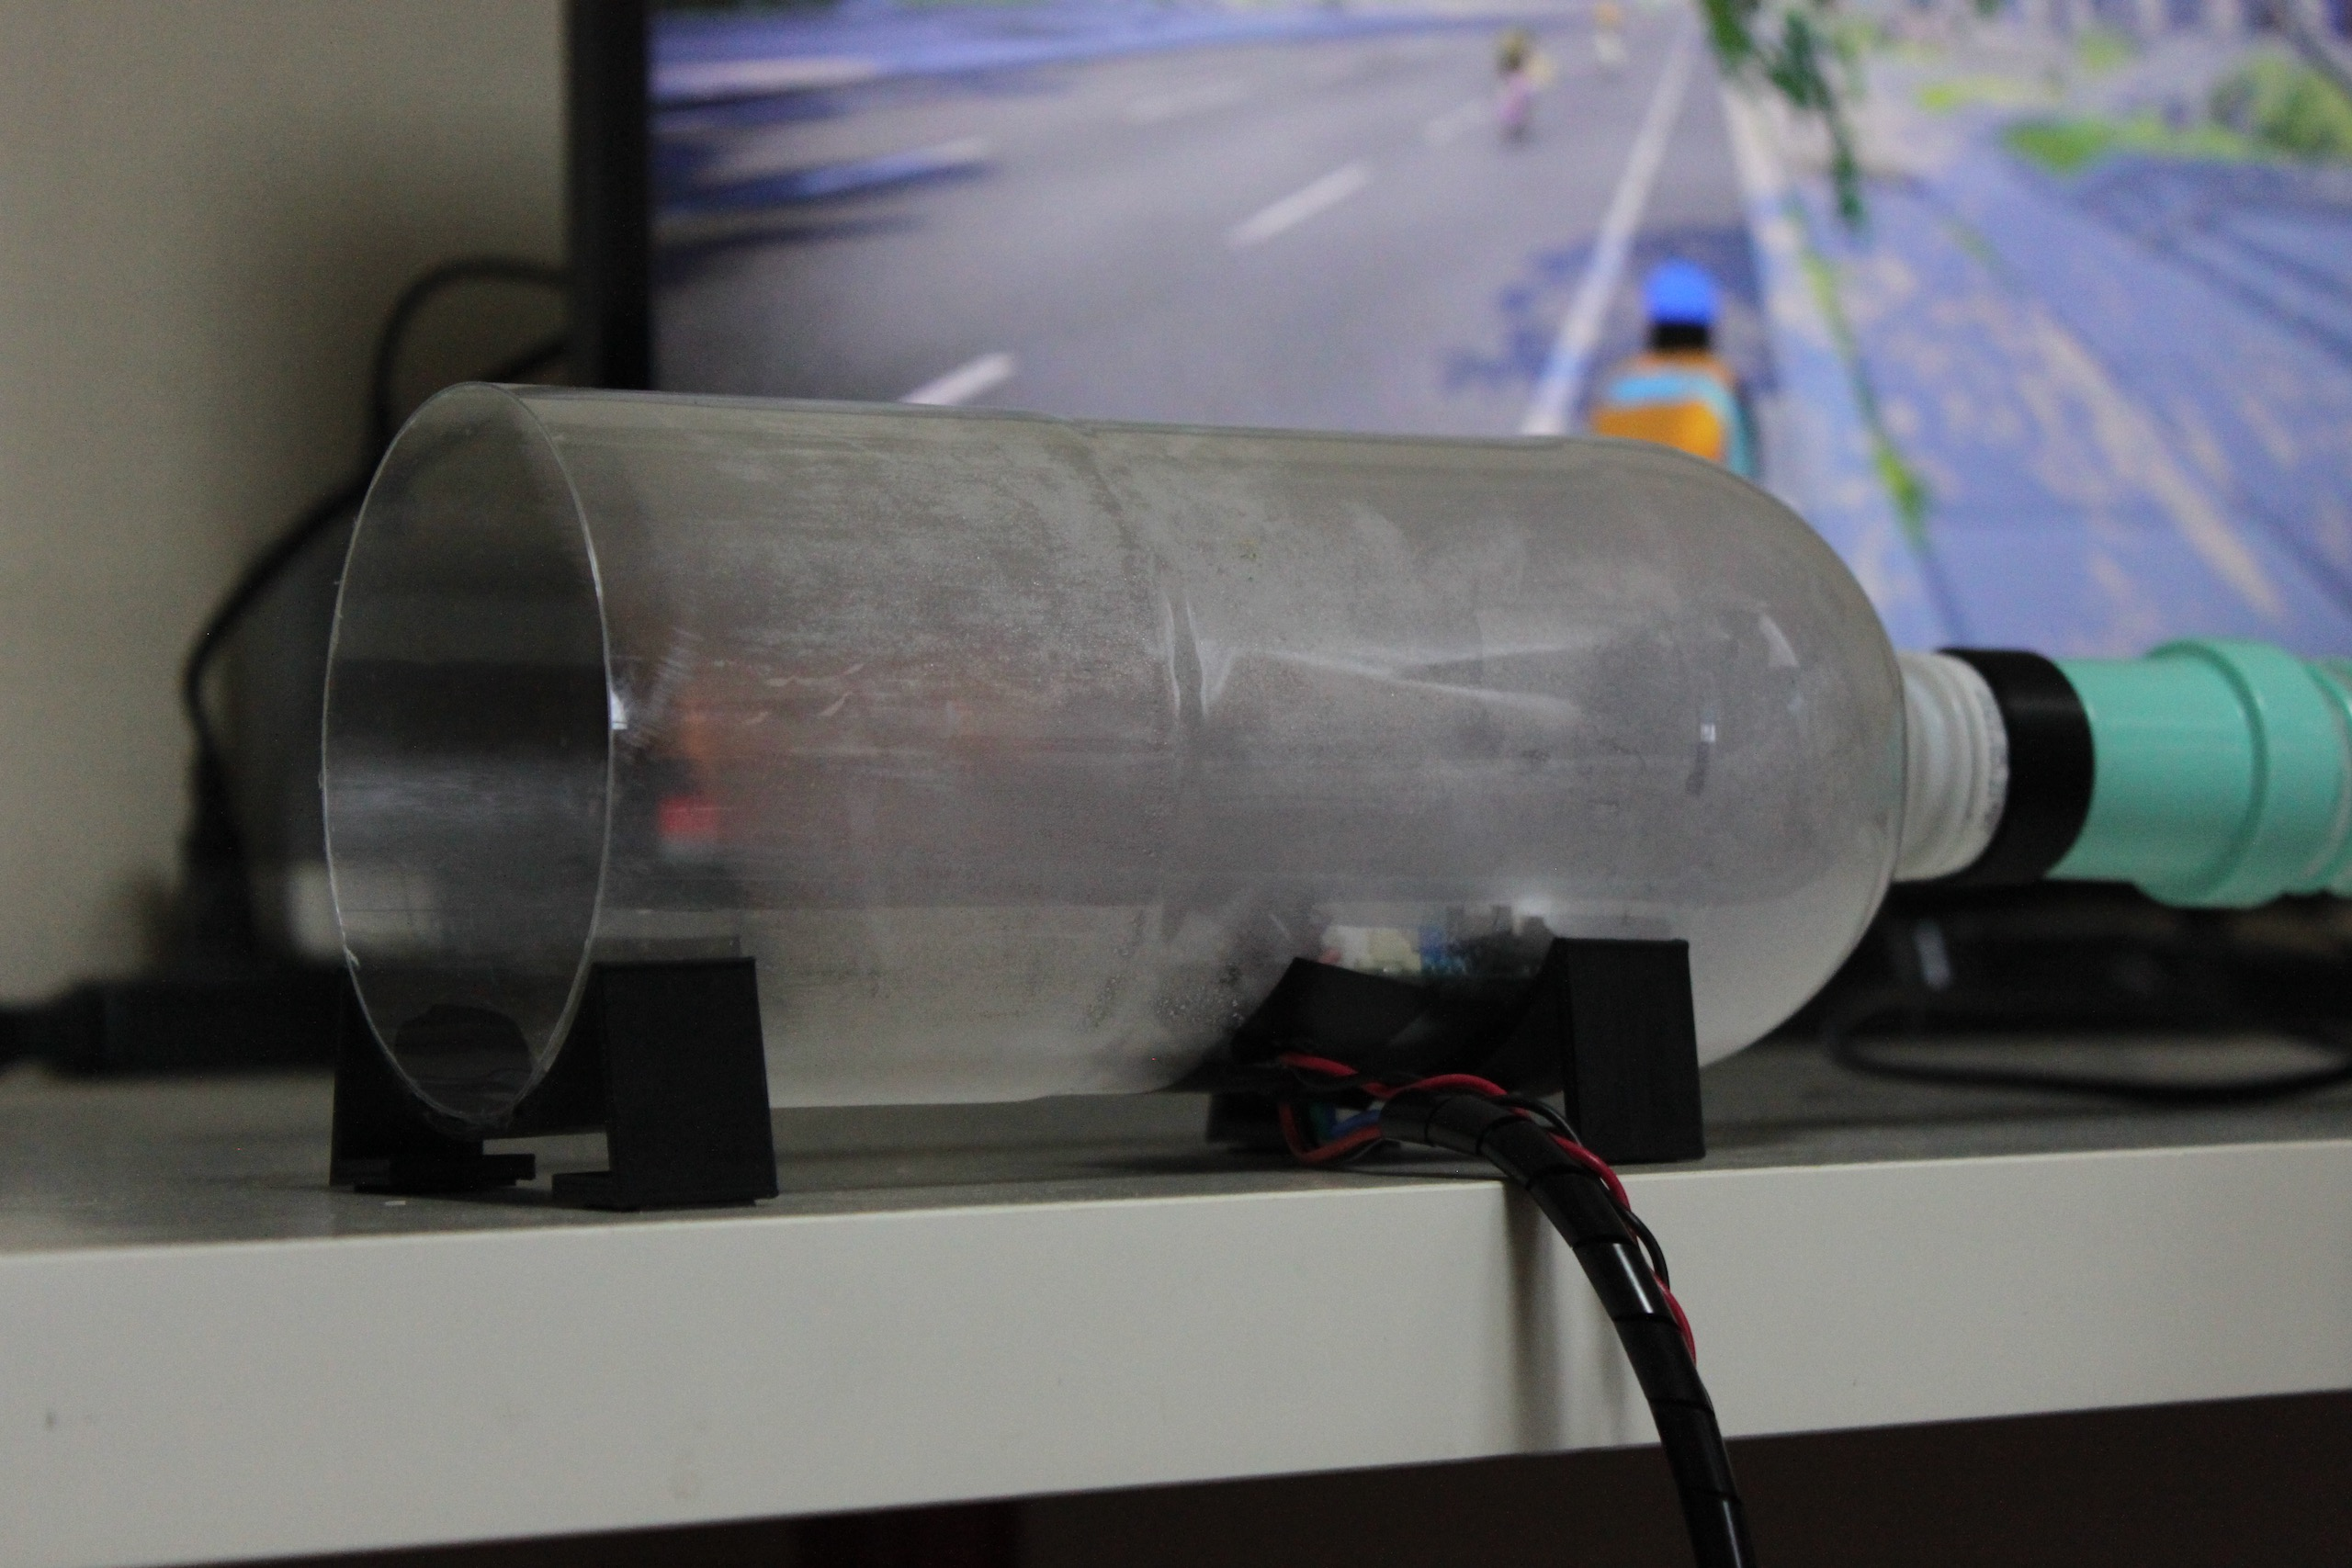
\includegraphics[width=8cm]{fig/mixing_chamber}
    \caption{製作したミキシングチャンバー}
    \label{fig:mixing_chamber}
  \end{center}
\end{figure}

図\ref{fig:mixing_chamber}は今回製作したミキシングチャンバーである.材料には入手のしやすさから1.5Lの炭酸飲料(CCレモン)のペットボトルを使用した.ミキシングチャンバーとホース(図\ref{fig:hose})を接合するためのジョイント部品はペットボトルのキャップ部のネジを使用し,ネジによる取り外し式としたものを3Dプリンターで製作した.

当初,ミキシングチャンバーは図\ref{fig:mixing_chamber_early}のように,チャンバー内のガス濃度の変化を小さくすることを意図して,ペットボトルのキャップ部同士を組み合わせて出口の流路を絞った形状としていた.しかし,実際に運動中の測定を行った場合,1分以内でチャンバー内の二酸化炭素濃度が二酸化炭素センサーの測定範囲を超えて上昇してしまうことが分かった.そこで測定中はガスの混合よりも極力外気との換気を図る必要があるということで,チャンバー内には特に障害物などを設けず,片側を解放した図\ref{fig:mixing_chamber}のような形状とした.

また,呼気ガスの成分のうち,二酸化炭素は気体標準状態において空気の2倍程度の密度があることから下方に滞留すると思われる.この際にミキシングチャンバーを置く方向が換気状況に大きく影響を与えることが予想されたので,今回はチャンバーを水平に保った状態で固定することとした.チャンバーとなるペットボトルを水平に保持できるようにするため,スタンド状の部品を3Dプリンターで製作し,センサー側の部品はネジ留めで,もう一方の部品はホットボンドで固定した.

\begin{figure}[H]
  \begin{center}
    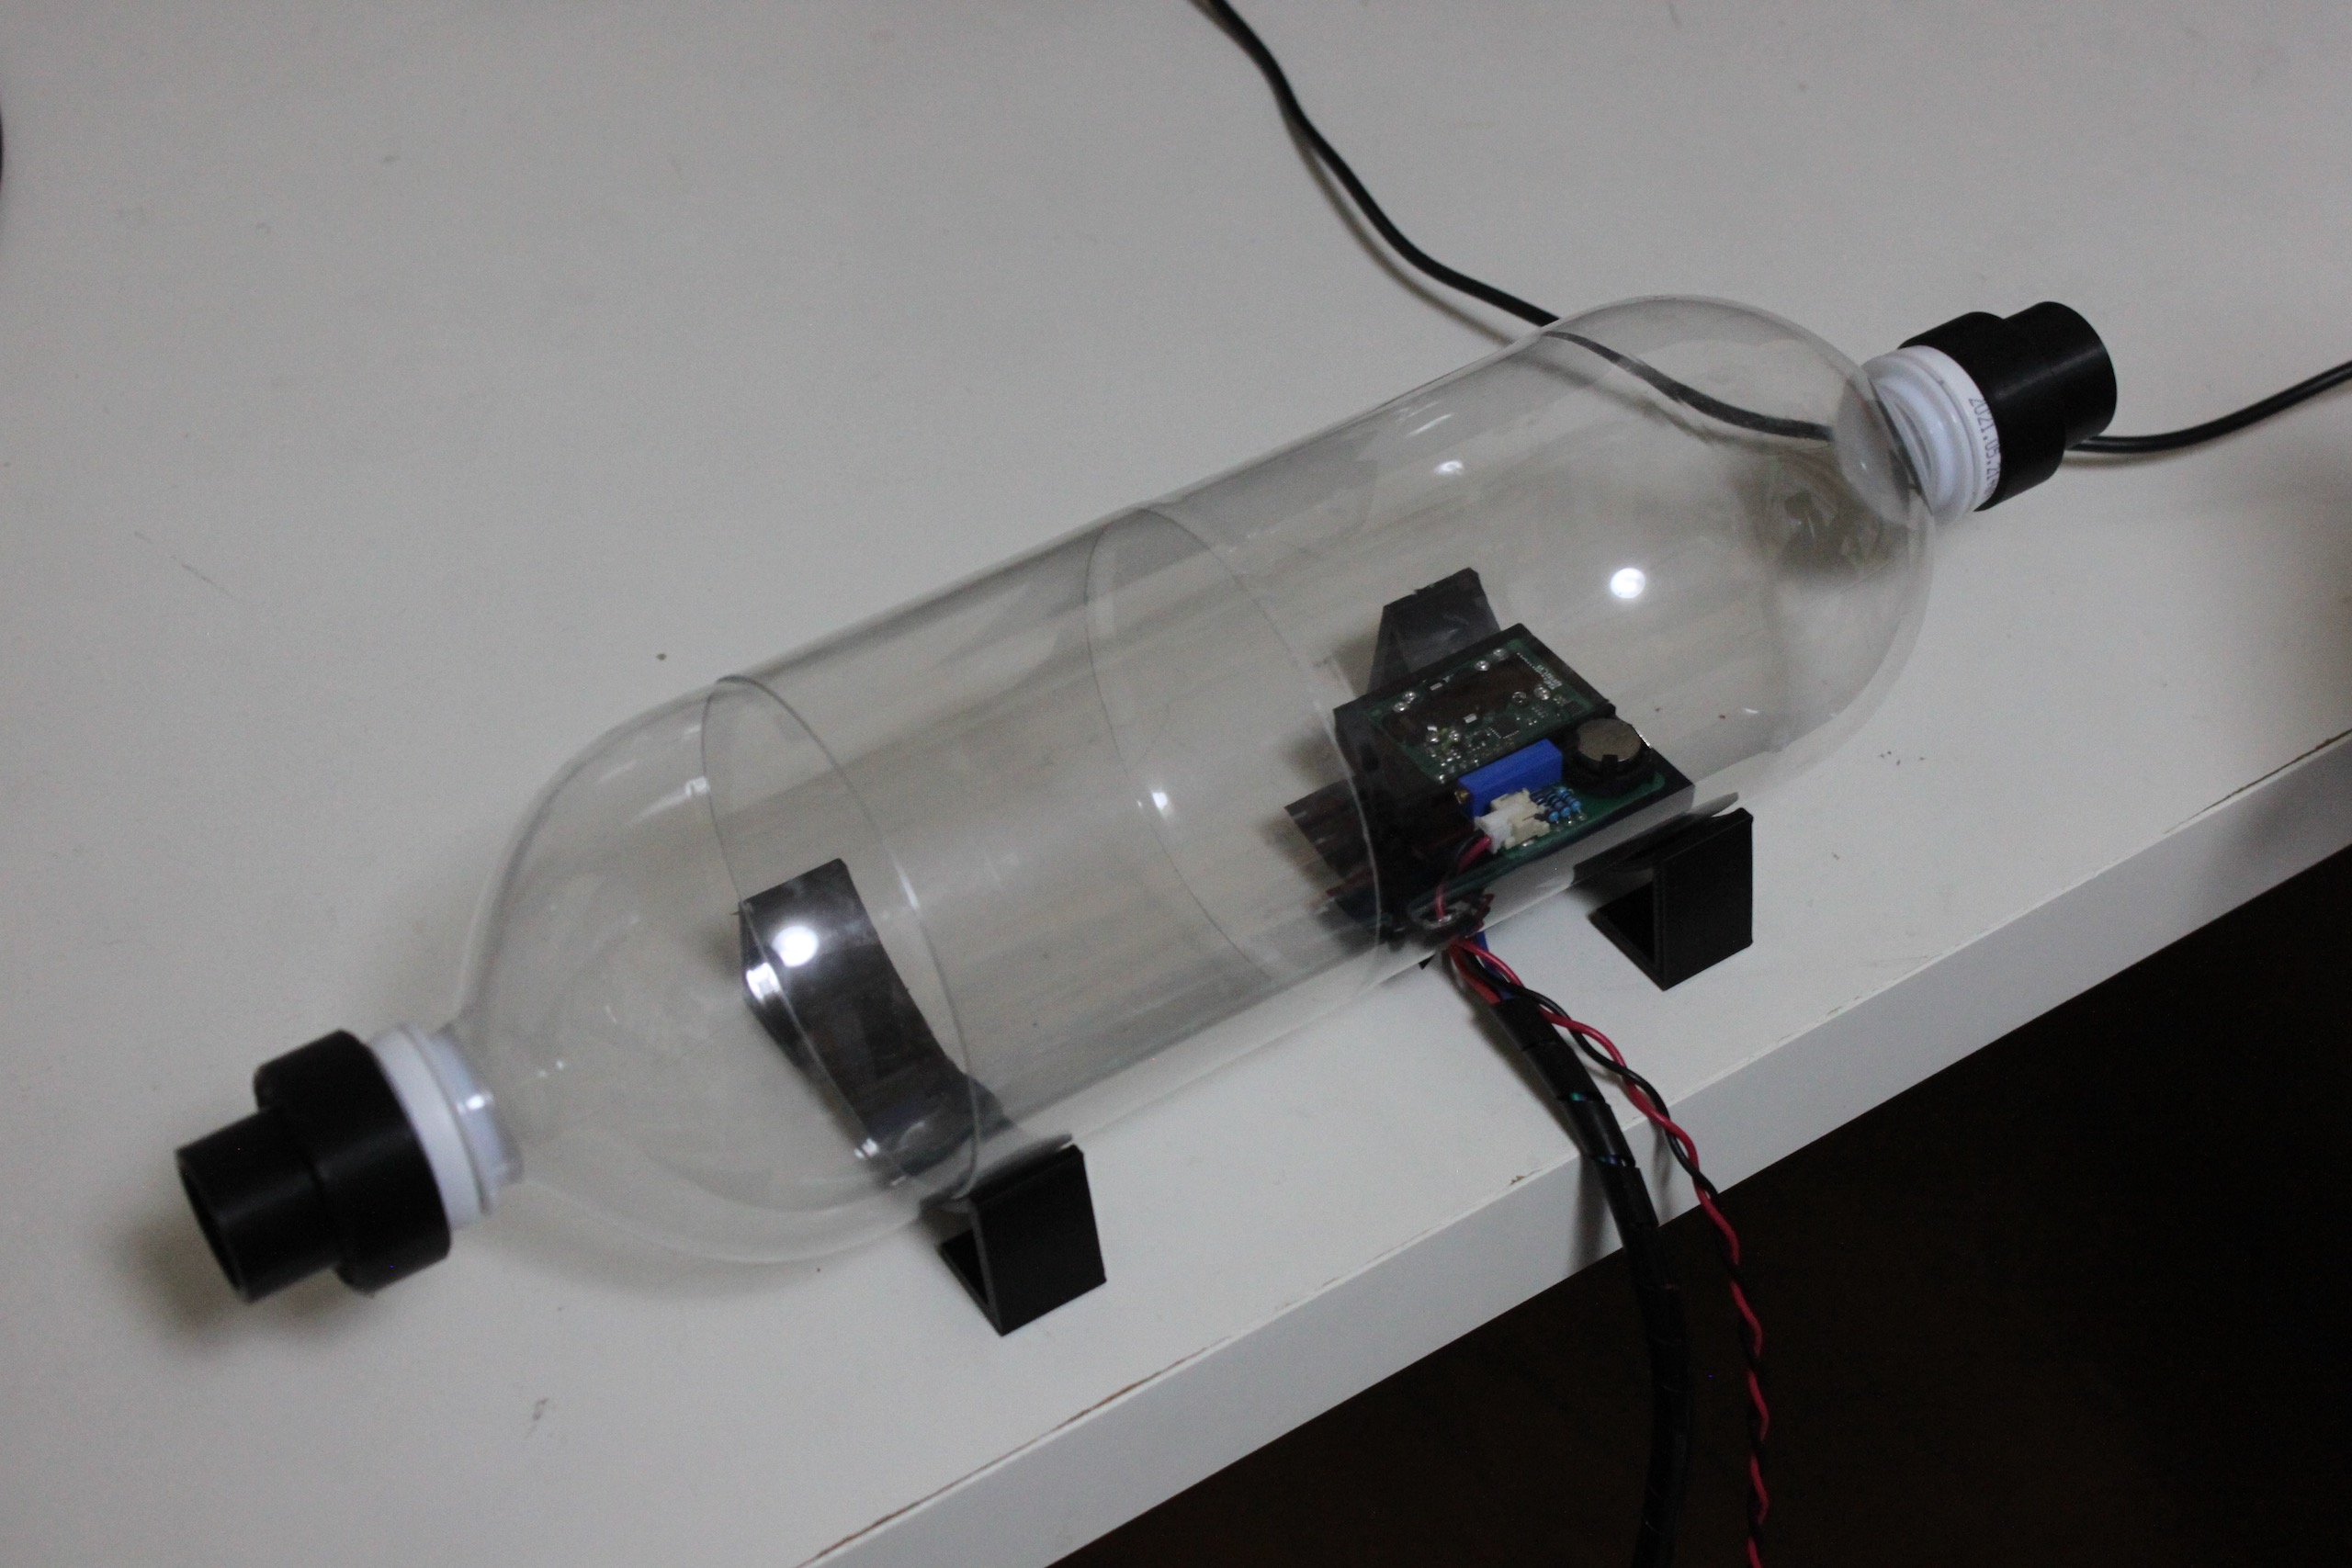
\includegraphics[width=8cm]{fig/mixing_chamber_early}
    \caption{当初のミキシングチャンバー}
    \label{fig:mixing_chamber_early}
  \end{center}
\end{figure}

\subsubsection{呼気収集マスク}

\begin{figure}[H]
  \begin{center}
    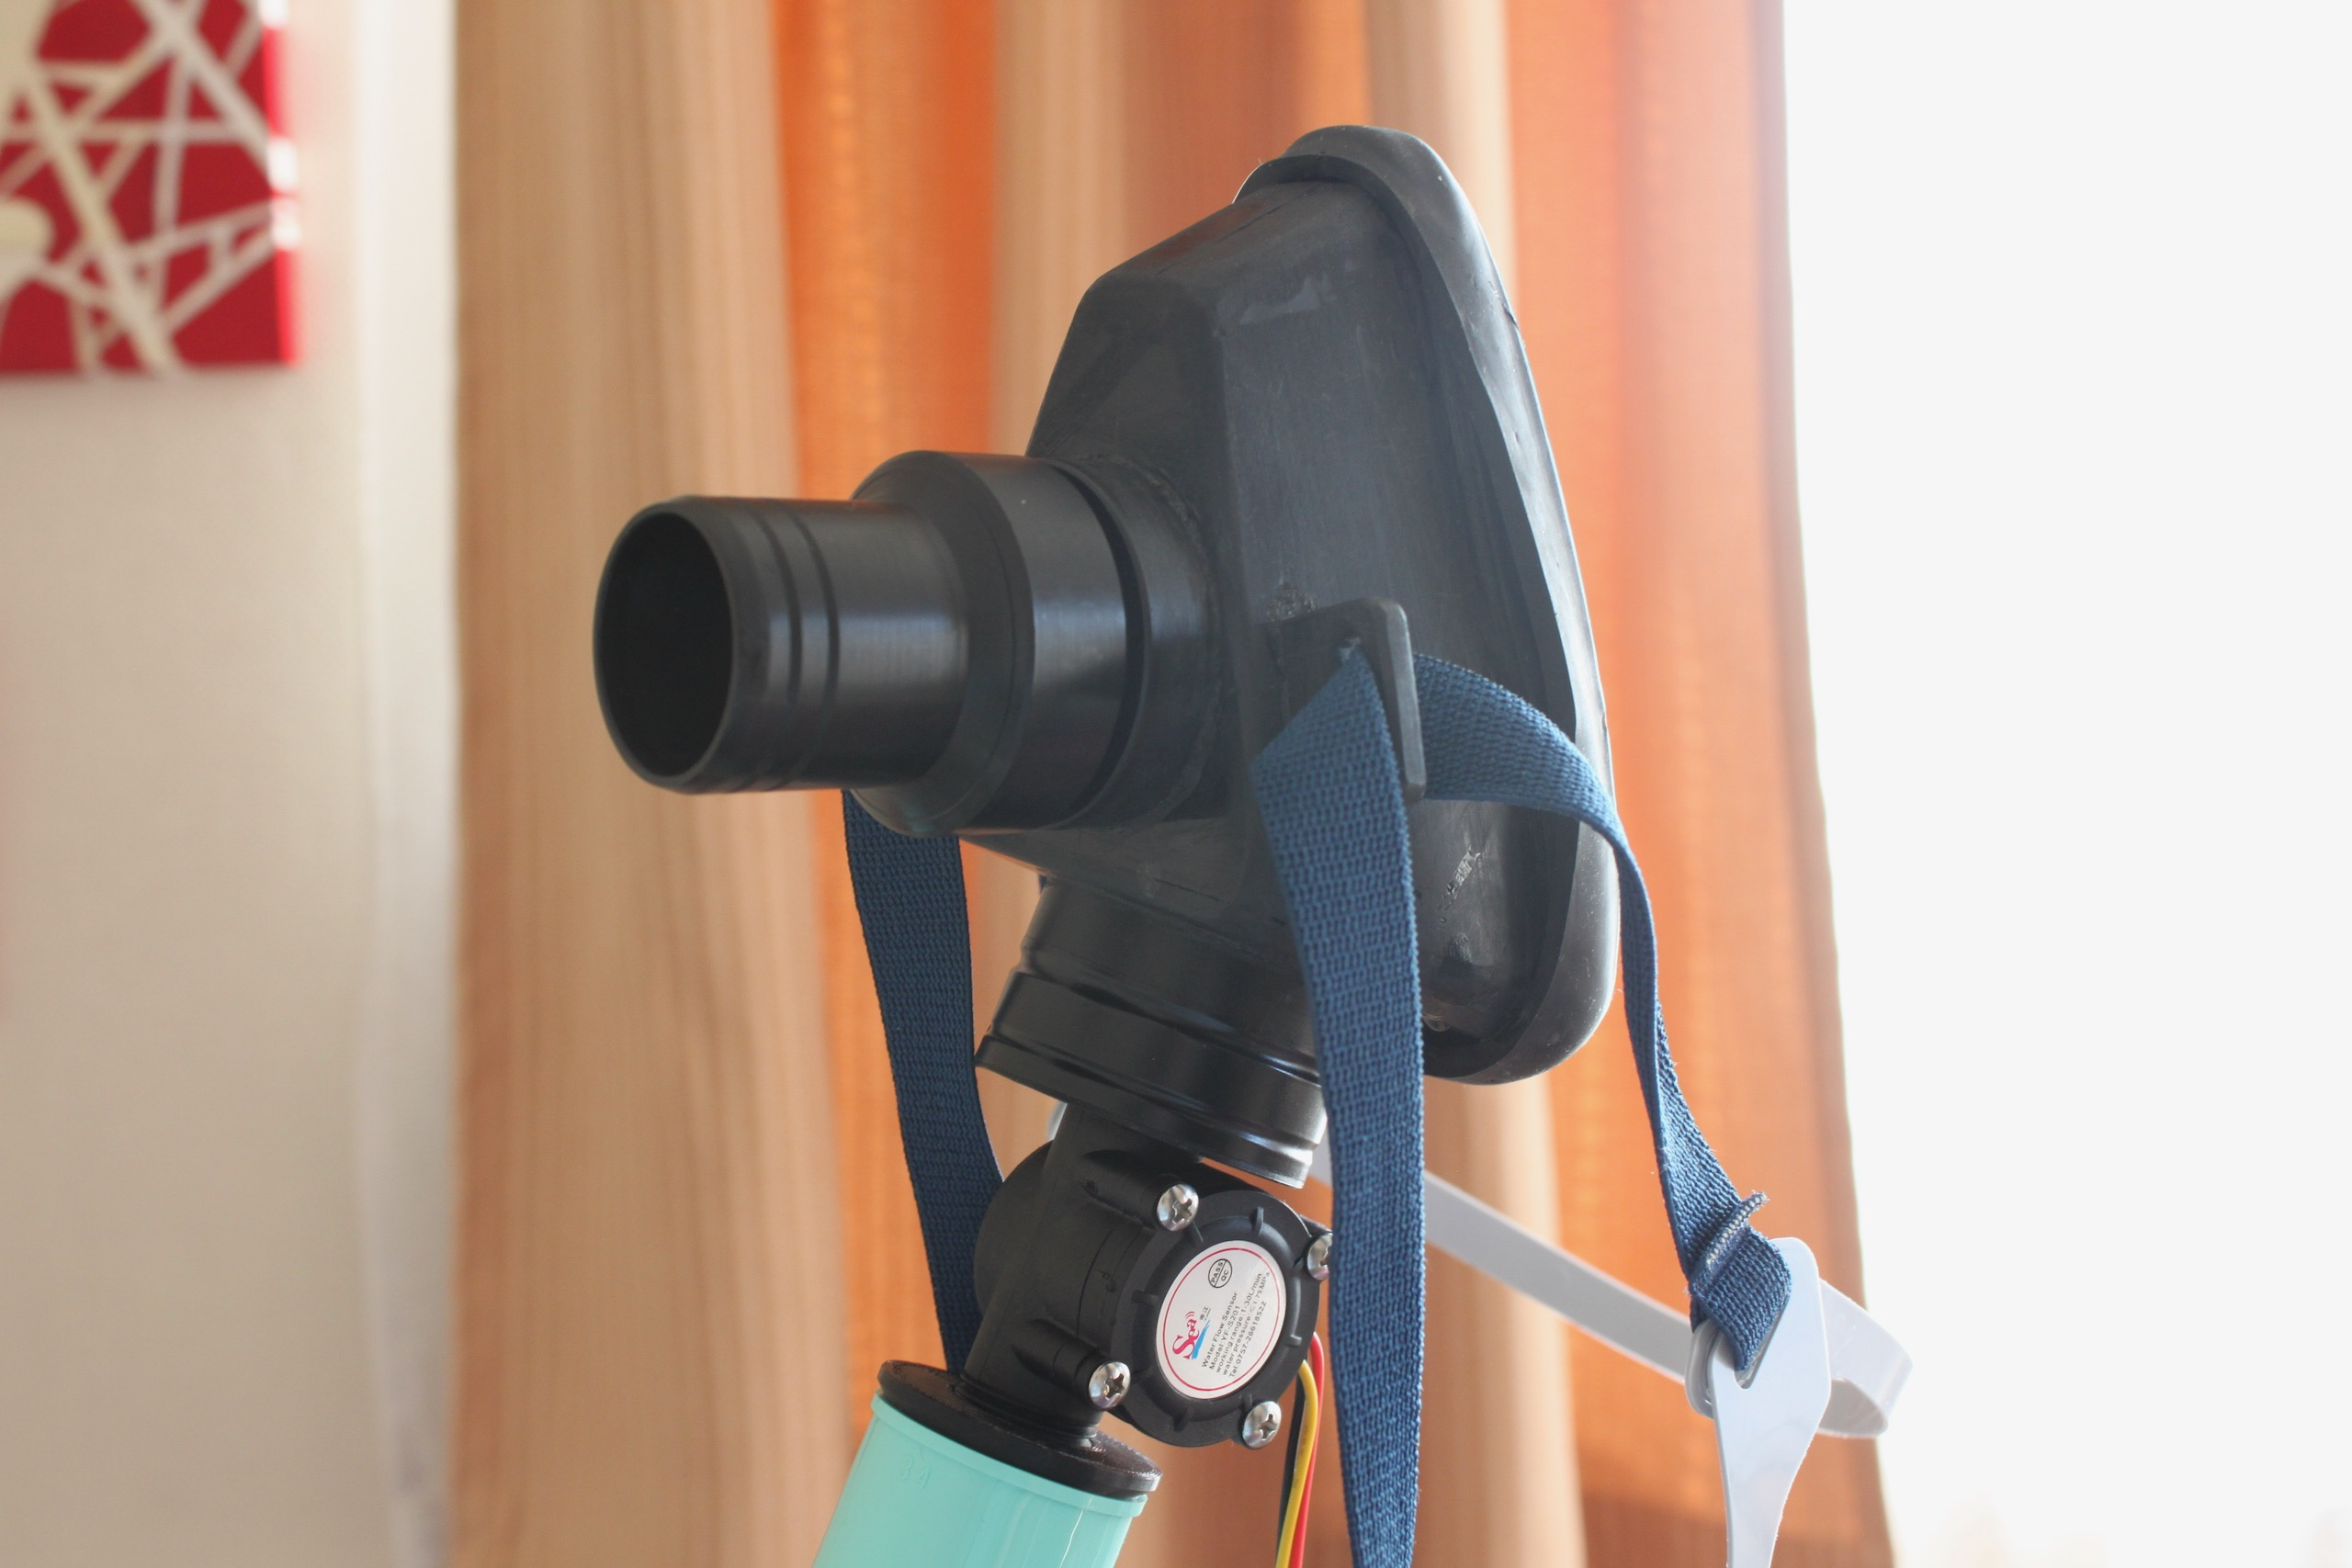
\includegraphics[width=8cm]{fig/mask_front}
    \caption{呼気収集マスク}
    \label{fig:mask_front}
  \end{center}
\end{figure}

呼気を収集するためには,呼吸の際の吸気と呼気を分離して呼気を収集するためのマスクが必要となる.これをここでは呼気収集マスクと呼ぶことにする.今回は呼気収集マスクには仰木研究室で以前に製作されたマスク(図\ref{fig:mask_front})を流用した.これは,アクリル板を組み合わせて顔に合うような形状を構成し,呼気及び吸気用の通気口を取り付けた物である.使用時に両手が使えるように,頭に固定するための市販のガスマスクから流用したバンドが取り付けられている.マスクの内側の顔に触れる部分には,顔との間にできる隙間を埋め呼気ガスが呼気の通気口以外から漏れ出すことを防ぐためのシリコーンゴム製のパッドが取り付けてある図(\ref{fig:mask_rear}).

\begin{figure}[H]
  \begin{center}
    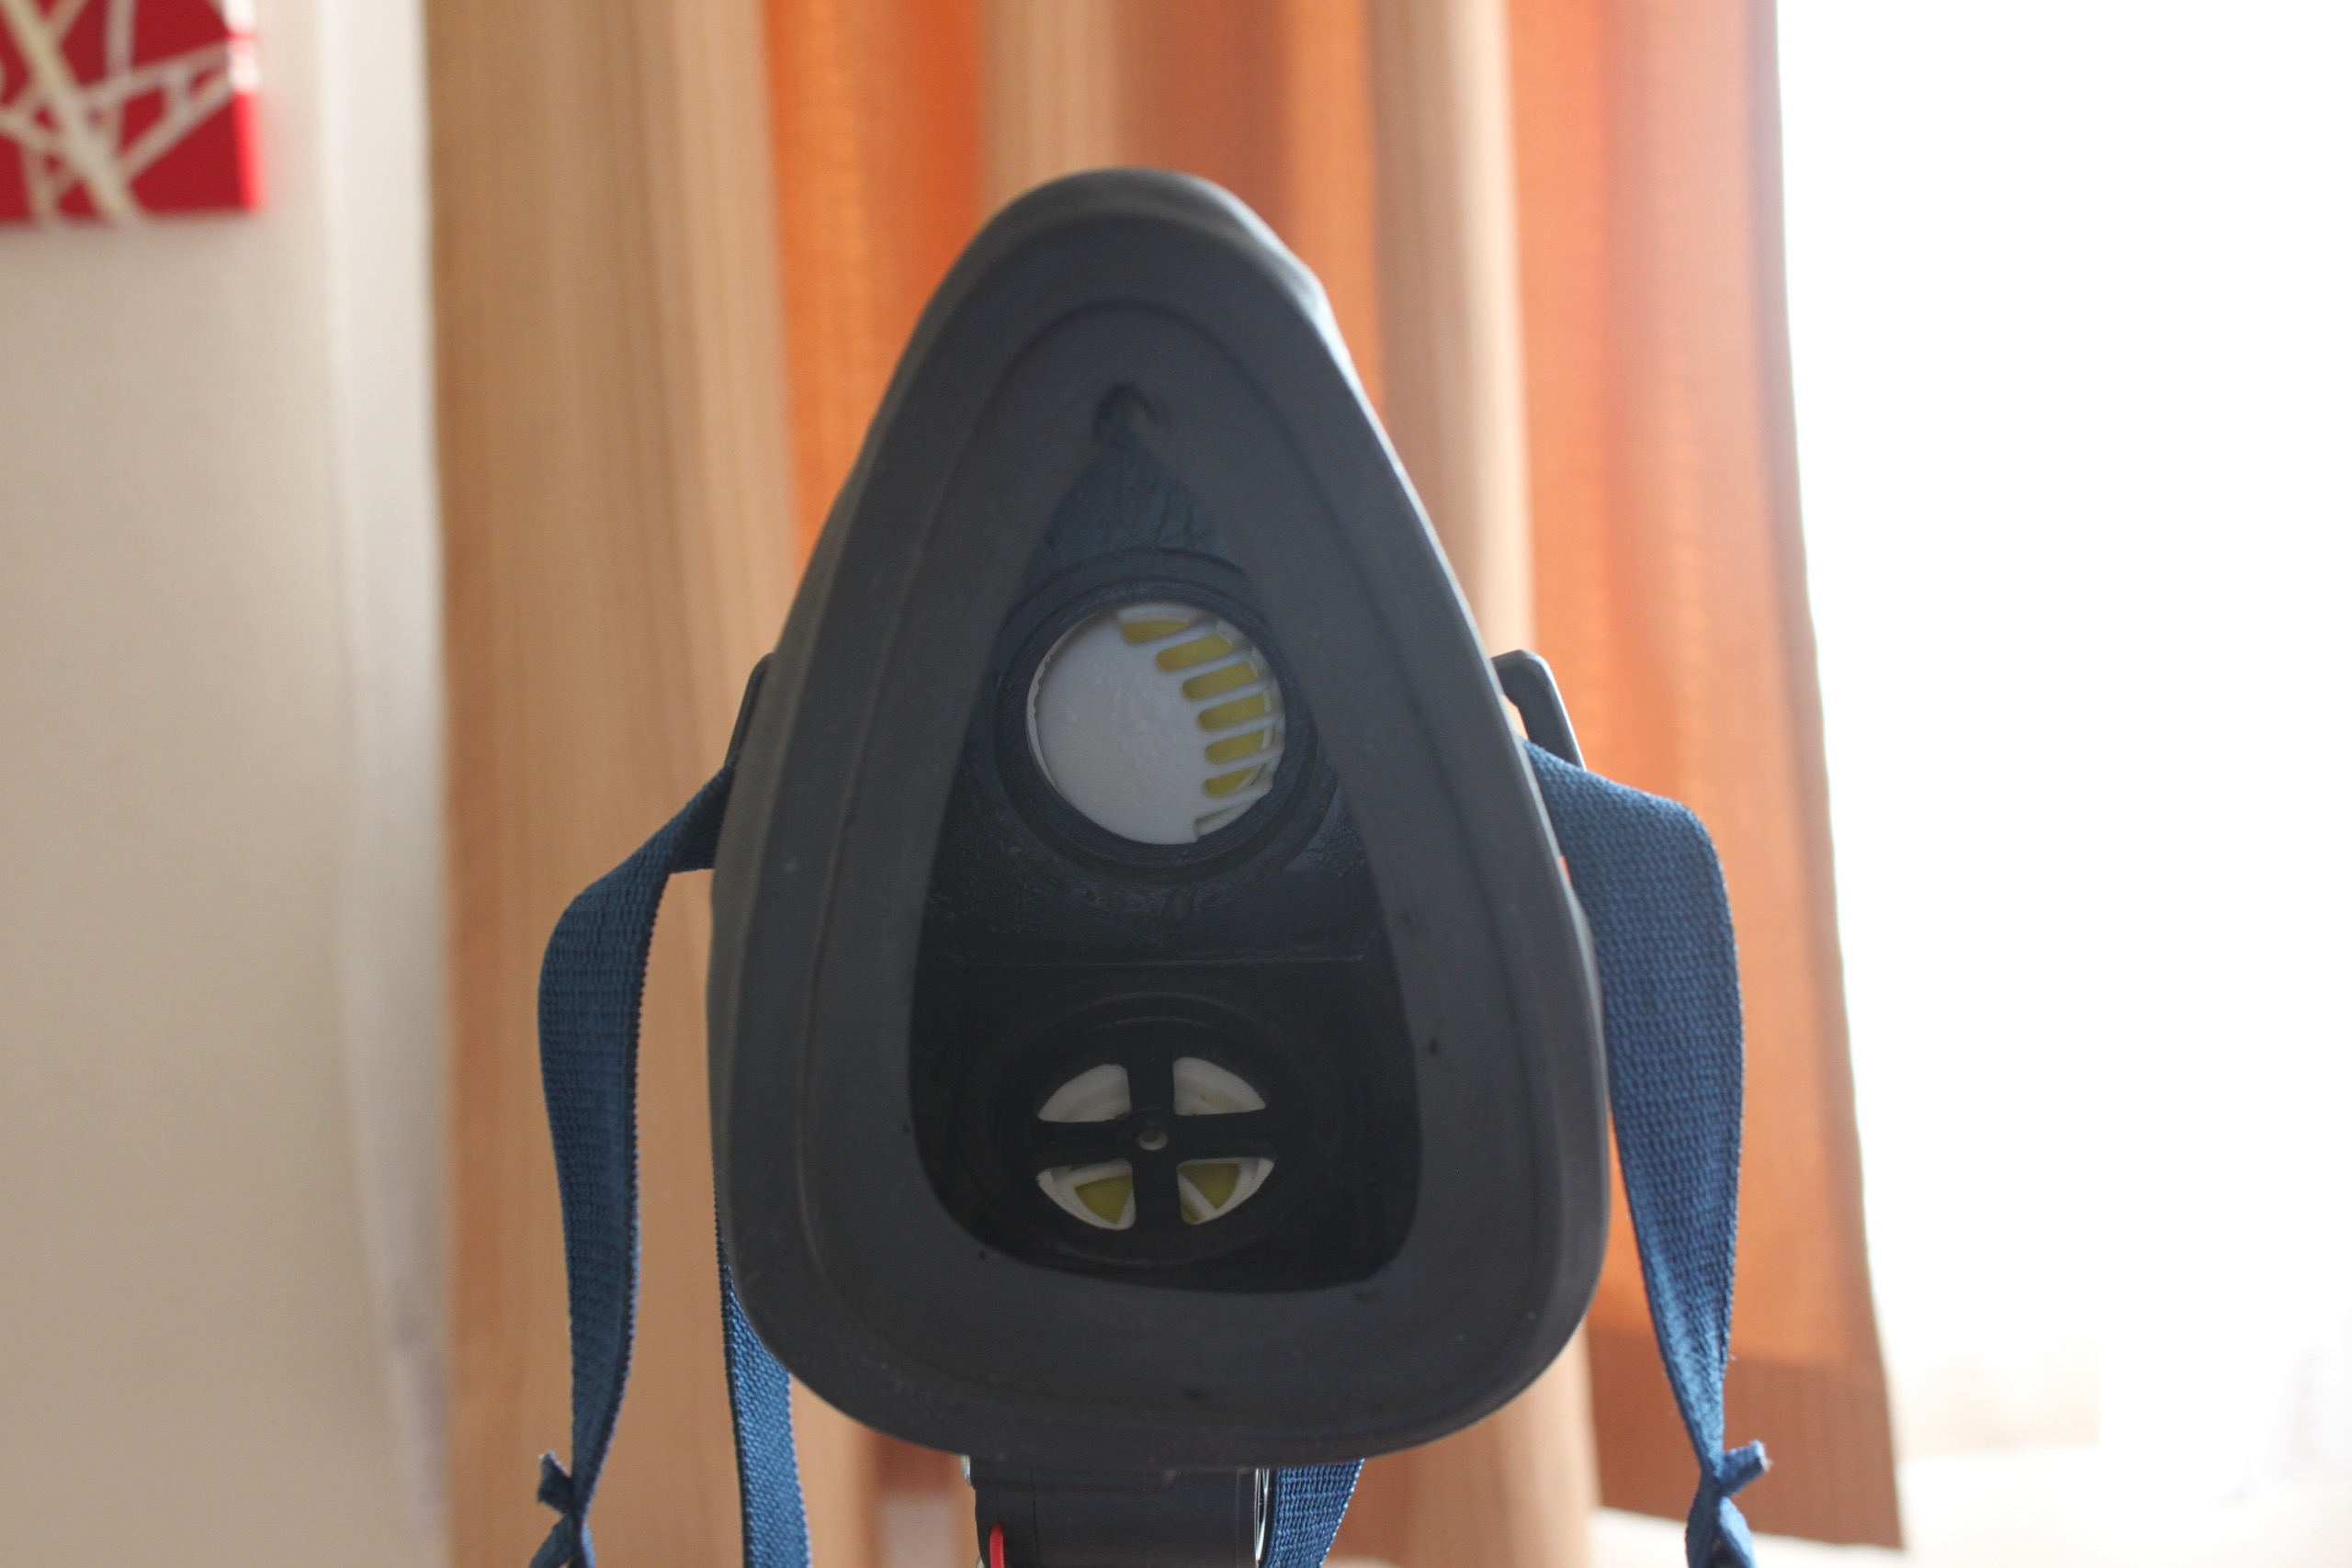
\includegraphics[width=8cm]{fig/mask_rear}
    \caption{内側から見た呼気収集マスク}
    \label{fig:mask_rear}
  \end{center}
\end{figure}

マスクの内側には,吸気と呼気を分離するために逆流防止弁を取り付けた(図\ref{fig:mask_rear}).今回使用した逆流防止弁は,運動時に使用するマスクに取り付けるために安価に市販されている物である.逆流防止弁の構造は図\ref{fig:bulb}のようになっている.ごく薄いシリコーンゴム製の膜は,一方向のみに捲れることができるようにプラスチック製の2つのパーツに挟まれて取り付けられている.これによって,弁を流れる気体の流れる方向を一方向に制限することができる.この弁を3Dプリンターで製作したスペーサーでマスク本体の径に合わせた上でネジで固定している.

\begin{figure}[H]
  \begin{center}
    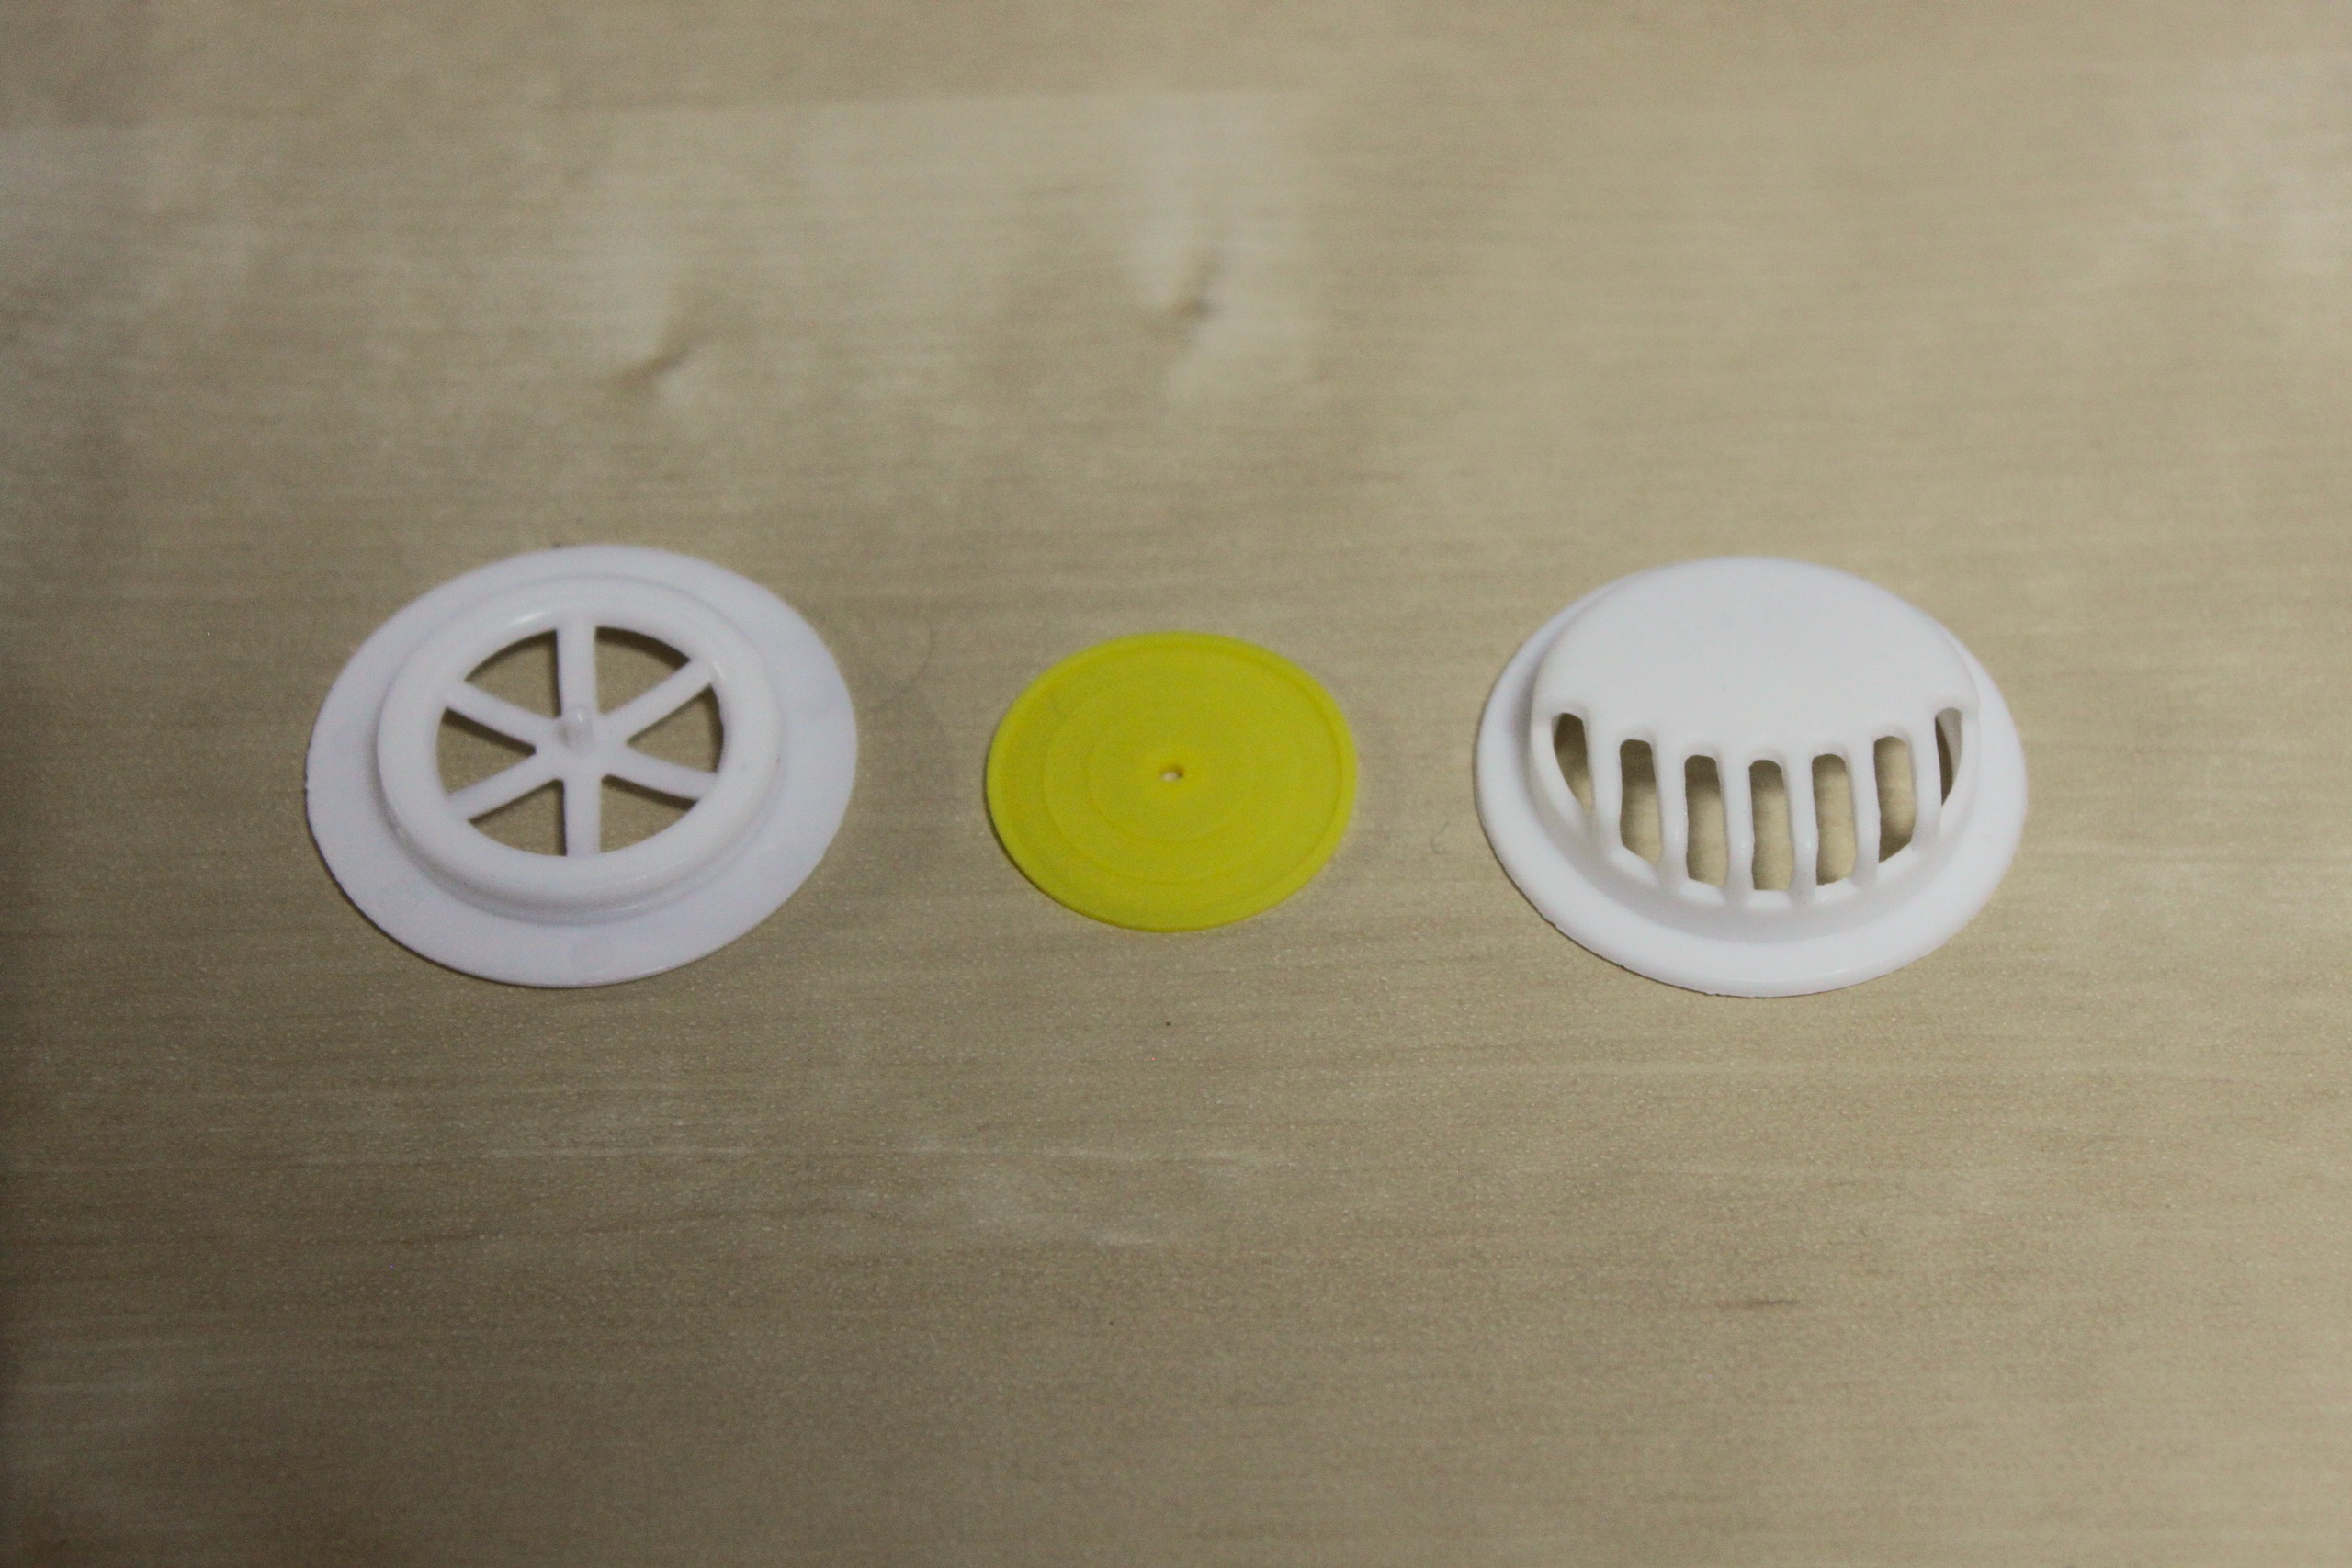
\includegraphics[width=8cm]{fig/bulb}
    \caption{逆流防止弁の構造}
    \label{fig:bulb}
  \end{center}
\end{figure}

ミキシングチャンバーと呼気収集マスクを接続するためのホースには,洗濯機の排水用ホースの延長ホースとして市販されている物(図\ref{fig:hose})を使用した.このホースは内径30mmの塩化ビニル製で,片側がゴム製,もう片側が硬質プラスチック製の継手となっている.今回はチャンバー側にプラスチック製,マスク側にゴム製の継手を接続することにし,ジョイント部品を3Dプリンターで製作した.

\begin{figure}[H]
  \begin{center}
    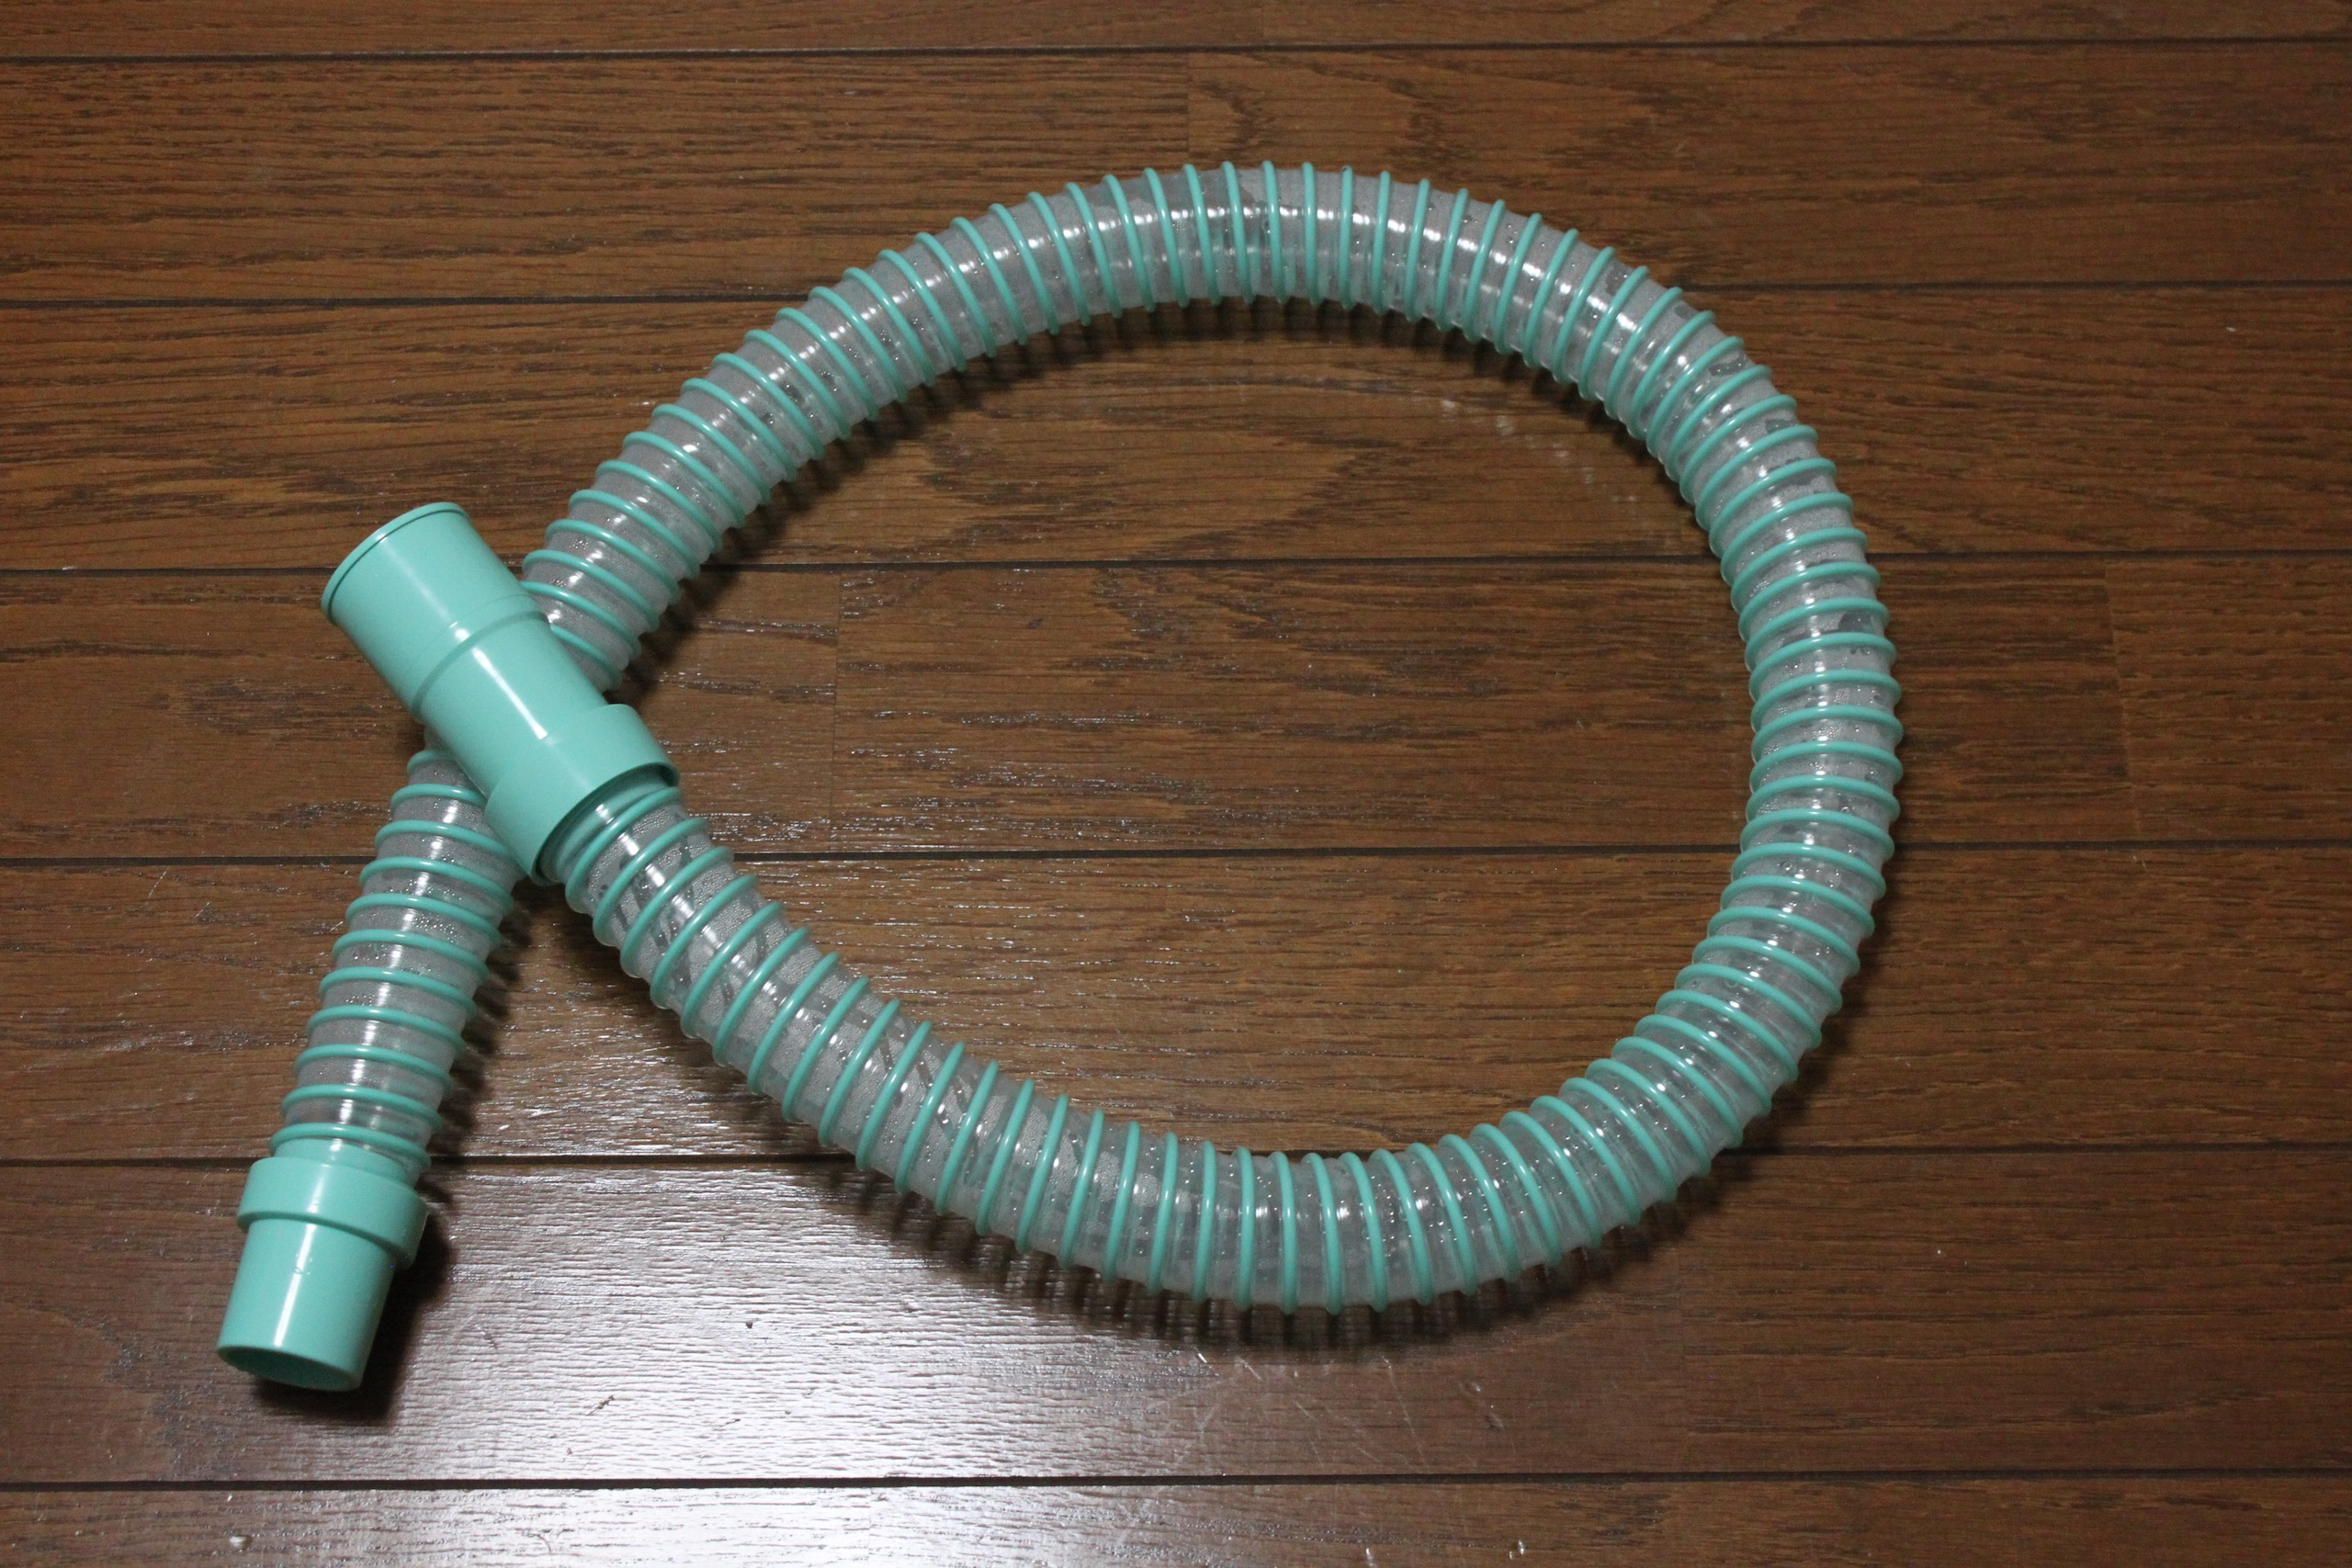
\includegraphics[width=8cm]{fig/hose}
    \caption{洗濯ホース}
    \label{fig:hose}
  \end{center}
\end{figure}

\subsection{換気量の測定}

\subsubsection{計測方式}

換気量V_Eを計測するための流量計には,マイコン工作用として市販されている水流計を使用した.

気体の流量を計測するための流量計の原理としては,差圧流量計と超音波流量計,タービン流量計などがある.差圧流量計は流路内に絞り機構を設け,その前後に発生する圧力差を測ることで流量を計測する方式である.超音波流量計は,流路内を流れる流体に超音波を照射することで流量を計測する方式である.タービン流量計は,流路にタービンを設置し,流体によって回転するタービンの回転数によって流量を計測する方式である.タービン流量計は単純な構造であり,他の方式に比べて微細ではない構造なので,水流計として安価に市販されている.呼吸代謝測定装置のうち,流量計は高価な部品であり,全体の価格を抑えるためにタービン流量計を使用した.

今回使用した流量計はYF-S201という名称で販売されているもので,流路に対してタービンの軸が垂直に取り付けられている接線流羽根車式のタービン流量計である.タービンの回転数に応じてホール素子が矩形波の信号を出力する.主な仕様を表\ref{tb:YFS201_specsheet}に示す.

\begin{table}[H]
  \begin{center}
  \caption{YF-S201 主な公称仕様}
  \label{tb:YFS201_specsheet}
    \begin{tabular}{lc}
      流路外径 & 20mm \\
      入口内径 & 9mm \\
      出口内径 & 12mm \\
      動作流量 & 1-30L/min \\
      関係式 & 1L_{水} = 450pulse
    \end{tabular}
  \end{center}
\end{table}

\subsubsection{タービン式水流計の流量関係式の算出}

仕様によれば,YF-S201は水流1Lあたりに450個の矩形波を出力する.これは水流が流れる時の値なので,空気の流量計として使用するためには空気が流れる際の関係式を求める必要がある.今回はこれを実験で求めた.

\begin{figure}[H]
  \begin{center}
    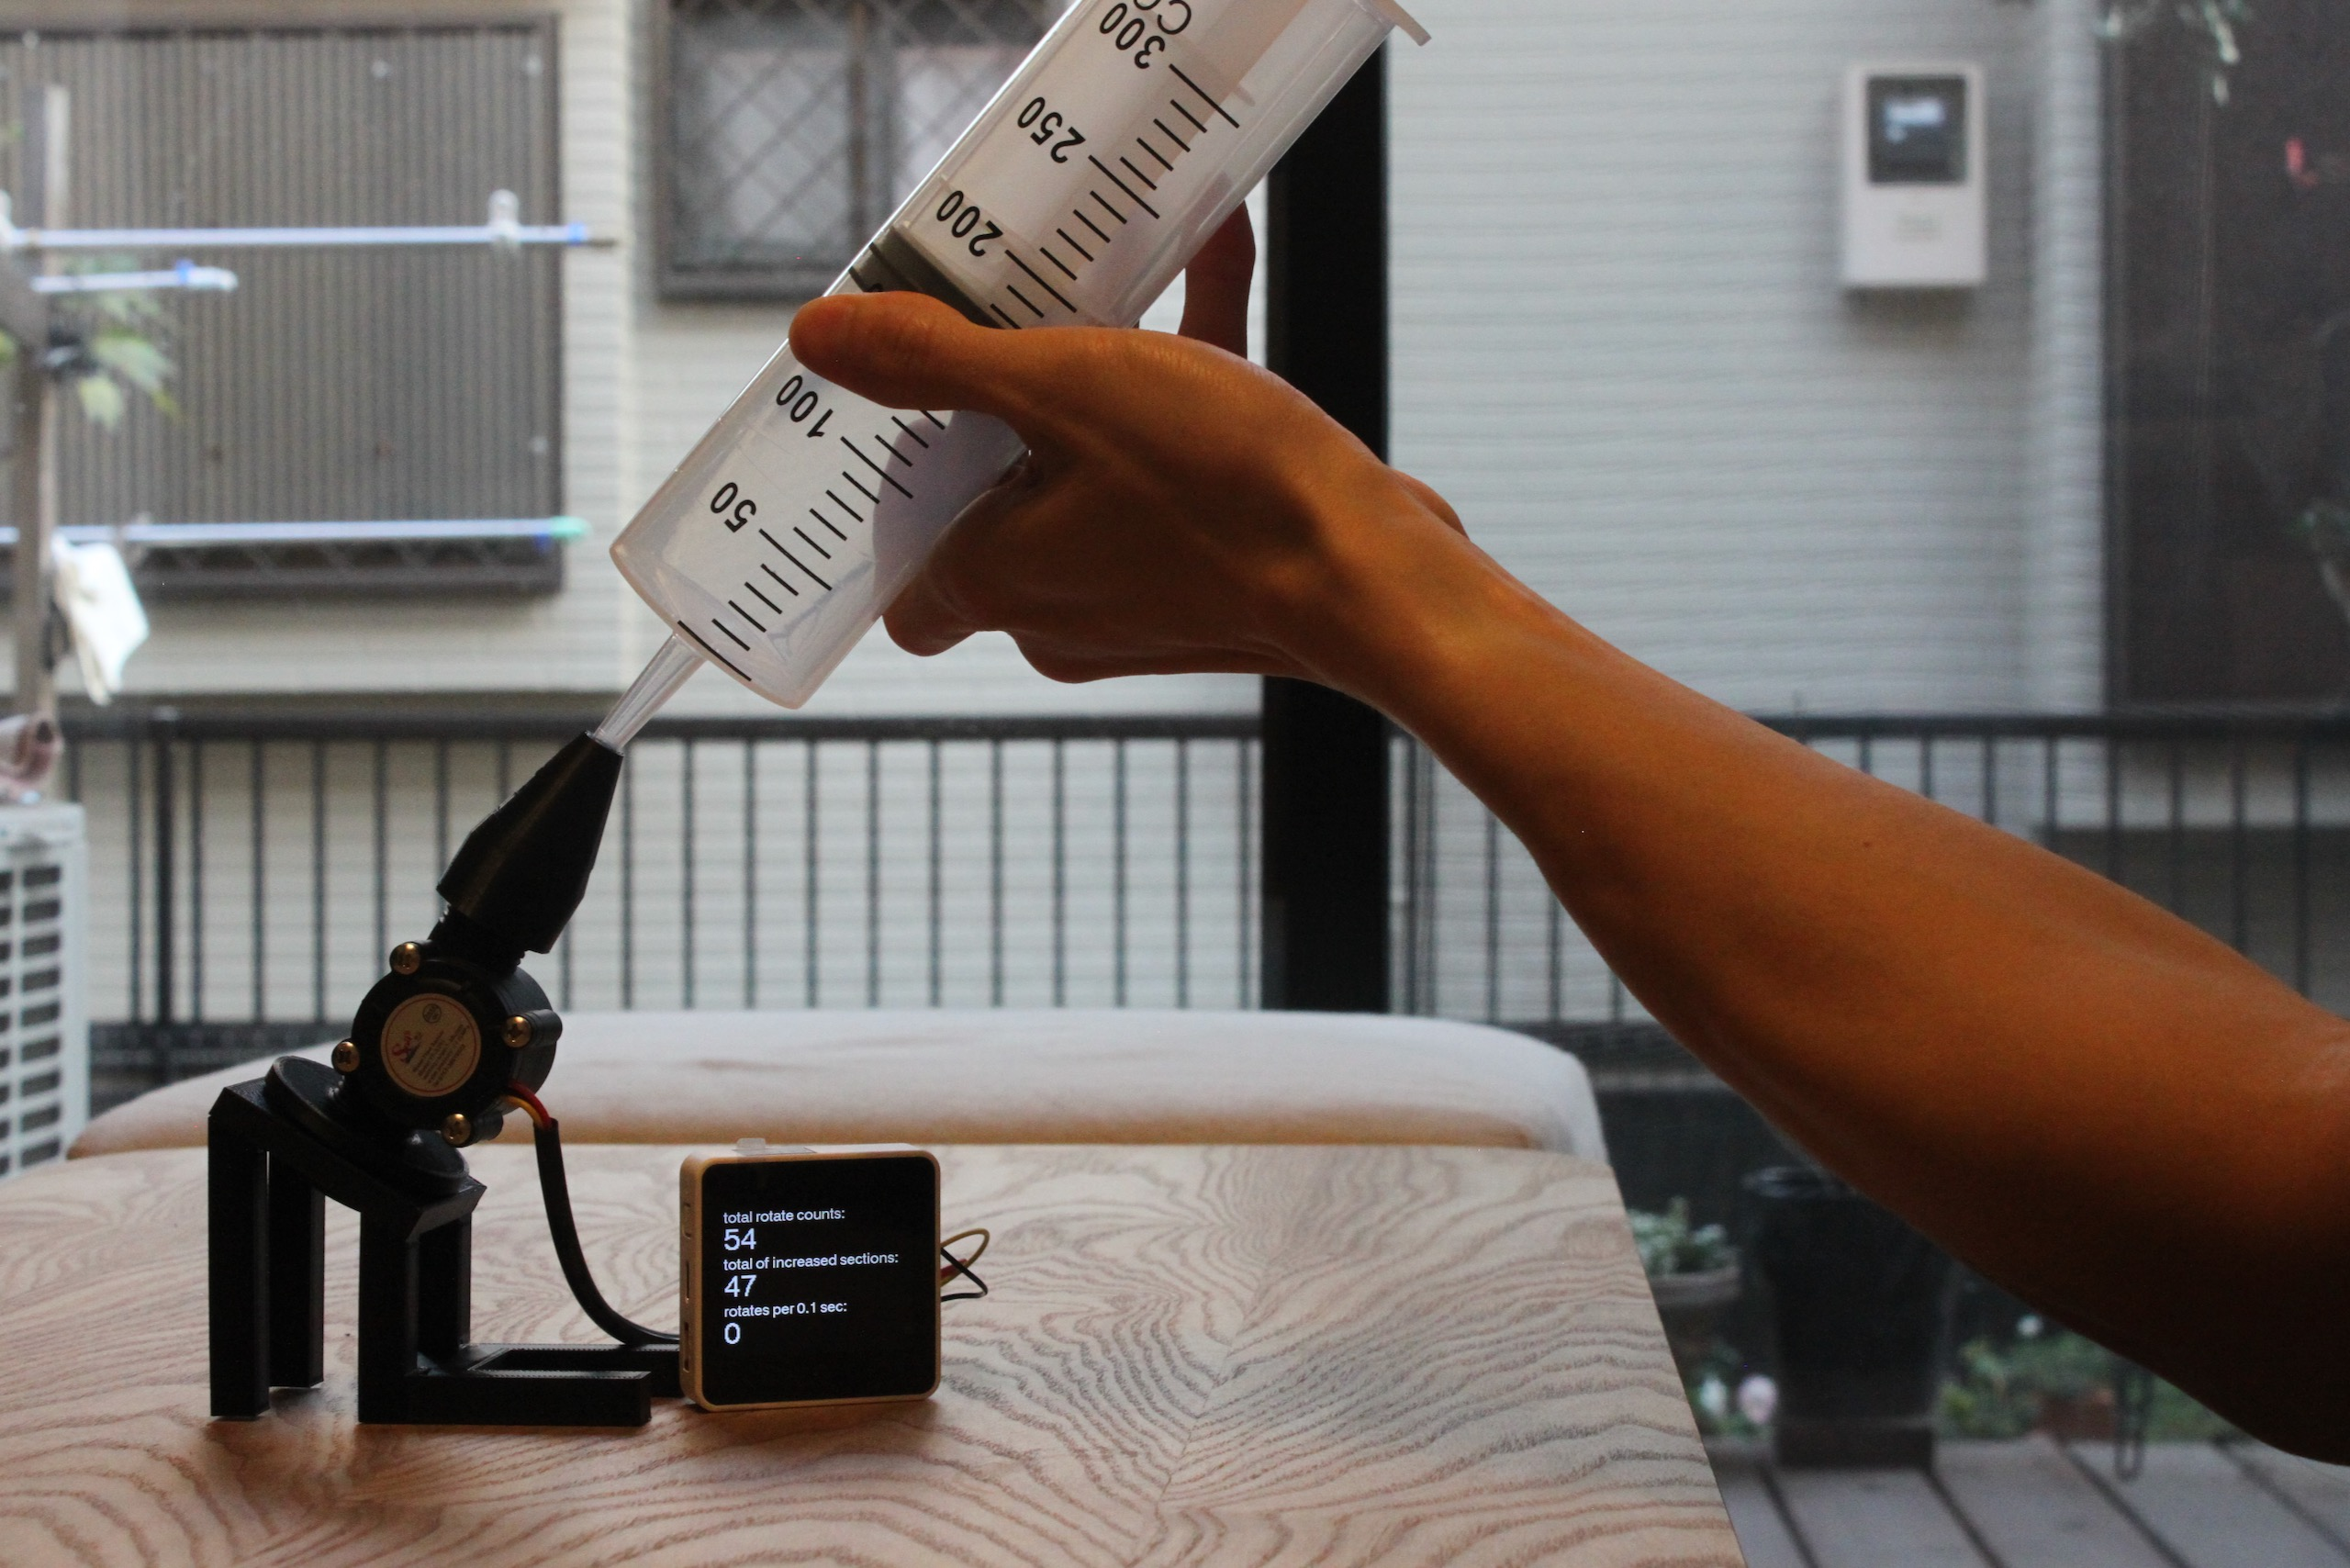
\includegraphics[width=8cm]{fig/flowsensor_calibrate}
    \caption{流量関係式算出用の実験}
    \label{fig:flowsensor_calibrate}
  \end{center}
\end{figure}

図\ref{fig:flowsensor_calibrate}は実験の全景である.
空気の量を正確に測りとれるシリンジを流量計の入り口に接続し,一定量の空気を送り込んだ時のタービンの回転数,すなわち矩形波の数を計測した.
送り込む空気の量は,入手が可能であったシリンジの最大サイズから300mLとした.シリンジのピストンを押す速さが出来る限り一定になるように注意しながら手でピストンを押した.シリンジと流量計の接続部は空気が漏れないようにするためにジョイント部品を製作した.シリンジのノズルと流量計のネジ部分を接続する部品を3Dプリンターで製作した.また,予備実験において,シリンジのノズルから出た高圧の空気が流量計のタービンの羽根に直撃すると回転数が多くなることが確認できたため,図\ref{fig:syringe_cone}のように,ノズルから出た空気が一度中央に当たってから流量計へと流れる形状とした.

\begin{figure}[H]
  \begin{center}
    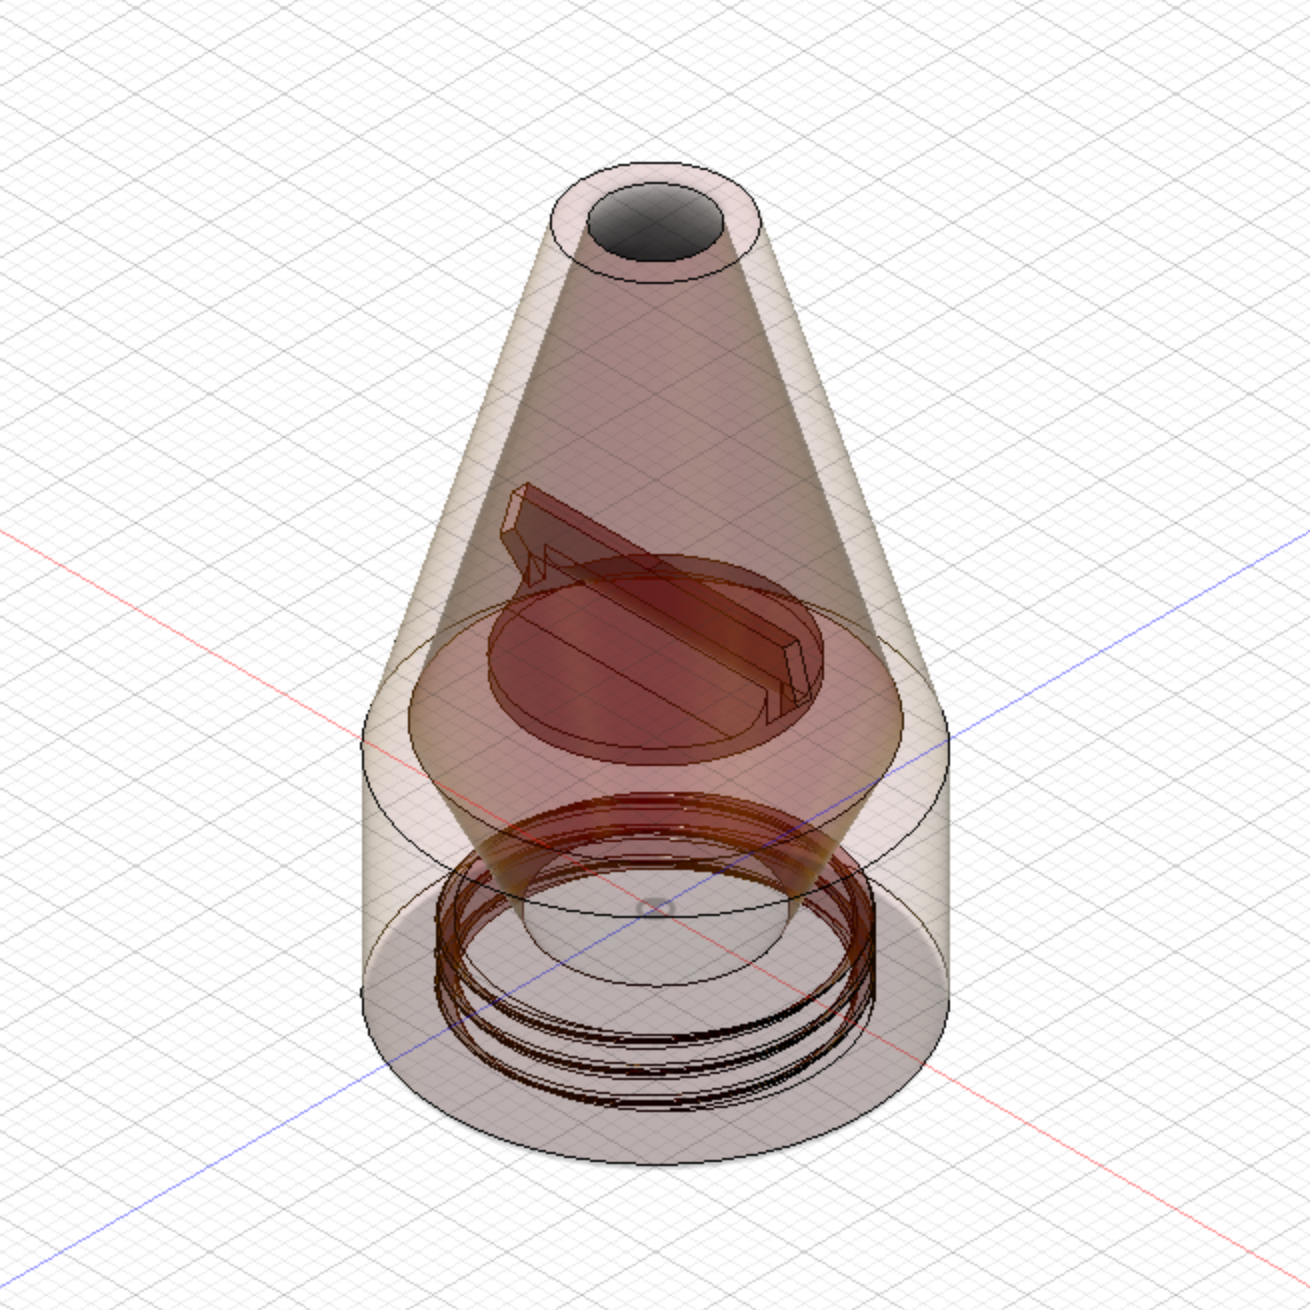
\includegraphics[width=8cm]{fig/syringe_cone}
    \caption{シリンジと流量計の接続用ジョイント部品}
    \label{fig:syringe_cone}
  \end{center}
\end{figure}

今回使用した流量計はタービン軸の回転の滑らかさが重力に影響されやすいことが予備実験から分かった.そこで,流量計の角度を実際にマスクに取り付けた際の顔を正面に向けた場合を想定し,60度に保持するための治具を3Dプリンターで製作した.
今回の装置では流量計は呼気側の逆止弁の排気側に取り付けられるため,呼気から吸気に切り替わった後も一定時間タービン流量計が空転する.正しく換気量を計測するためにはこの空転分の回転数を除外する必要がある.そこで,回転数を計測するプログラムにこれを除外する処理を加えた.0.1秒毎の回転数を計測し,一個前の区間と比べて値が減少している区間の回転数を除外するという方法で行った.
以上の処理を行い,空転分を除外した回転数を計測するプログラムをM5Stack Core2で動作させ,200回分のデータの代表値を0.3mLの空気が流れた時の回転数とするという方法で流量関係式の算出を行った.結果は以下の通りである.

ミキシングチャンバー方式で換気量を測定するため,マスクの呼気方向にのみ解放される弁の先に取り付けた流量計で換気量を測定する

今回はマイコンなどに接続する水量計として安価に市販されているタービン流量計を流量計に用いた.YF-S201という名称で販売されているもので,タービンの回転数をホール素子センサーによって測定するものである.

呼気のような微小な気体の流量を測定するための流量計には,差圧流量計,超音波流量計,タービン流量計などが用いられる.

差圧流量計は,流路内に絞り機構を設置し,その前後に設置した圧力計から得られる圧力差から流量を測定する方式である.絞り機構としてオリフィスプレートを用いたものはオリフィス流量計と呼ばれる.
超音波流量計は流路内を流れる流体に超音波を照射することで流量を測定する方式である.
タービン流量計は流路にタービンを設置し,流体によって回転するタービンの回転数によって流量を測定する方式である.

%差圧流量計は,流路内に絞り機構を設置し,その前後に設置した圧力計から得られる圧力差から流量を測定する方式である.絞り機構としてオリフィスプレートを用いたもの(オリフィス流量計)はCardioCorchやVO2000などの既存の呼吸代謝測定装置で使用されている.

%超音波流量計は流路内を流れる流体に超音波を照射することで流量を測定する方式である.高精度が特徴であり,NASAが開発したPUMAに使用されている.

既存の呼吸代謝測定装置の流量計には主に先述の三方式が用いられるが,今回は水流センサーとして汎用的に安価に入手が可能であるということでタービン流量計を用いた.

\subsubsection{信号処理}

数値計算に必要な換気量は1分値であるので,タービンの回転数の計測時間を長くすることによって誤差を減らすために1分毎に1分間の合計のタービンの回転数を係数で割った値を現在から1分前の区間の換気量としている.画面表示用の瞬間換気量は1秒毎の回転数を係数で割ったものだが,これは数値計算には用いていない.

\subsection{呼気酸素濃度の計測}

\subsubsection{空気亜鉛電池式センサー}

今回は株式会社ピーバンドットコムから発売されている「実習用酸素センサキット A-5S」(以下「A-5S」)を酸素センサーとして使用した.A-5Sは,補聴器など用に汎用的に使用される空気亜鉛電池をセンサーとして使用し,空気亜鉛電池の出力電圧から酸素濃度を測定するというセンサーで,組み立てキットとして1000円程度で購入が可能である.構造は単純であり,空気亜鉛電池に固定抵抗と可変抵抗を接続したというものである.キャリブレーションは大気中の酸素濃度20.84\%とに合わせて出力電圧が20.84mVになるように可変抵抗を調整して行う.空気亜鉛電池の電圧の低下から,長時間連続での測定は困難である.

従来,呼吸代謝測定装置の酸素センサーにはガルバニ電池式センサーが多くの場合で使われてきた.この方式は高精度であるが,酸素濃度に応じて電圧を出力することで酸素濃度を測定するためのガルバニ電池が10000円以上と高価であるため,安価に入手できる空気亜鉛電池をセンサーとして用いたA-5Sを使用した.

\subsubsection{信号処理}

A-5Sが出力する電圧は酸素濃度21\%時に21mVと非常に微弱である.この電圧を今回使用したマイコン,M5Core2(ESP32)の12bit ADコンバーター(0-3.3V, 4096段階)で測定するために,アペアンプを使用して増幅した.オペアンプには,単電源のフルスイングオペアンプNJM2732Dを用いた.非反転増幅回路を用いてA-5Sの出力電圧を101倍に増幅し,酸素濃度21\%時に2.1V程度に増幅することで測定精度を高めている.
なお,NJM2732Dは2回路入りのオペアンプであるため,接地を兼ねてもう一回路分のターミナルも結線している.現時点では呼気酸素濃度F_EO_2用の一つしか使用していないA-5Sをもう一つ追加し,吸気酸素濃度F_IO_2を計測することも可能である.

A-5Sが出力する電圧をオペアンプで増幅し,M5Stack Core2のADコンバーターで読み取ったところ,周期的にスパイク状に高い値を出力していることが確認できた.これを取り除くためにプログラム上のデジタルフィルターで信号を平滑化した.今回使用したのは移動

(回路図)

\subsection{呼気二酸化炭素の計測}

呼気二酸化炭素濃度は運動負荷によって変化し,安静時の約1\%から高強度運動時には9\%まで変化するという\cite{co2_percent}.そのため,運動中の呼吸代謝の測定にはこの範囲の二酸化炭素濃度の測定に対応する必要がある.

ところが,1万円程度以下で入手可能な市販の二酸化炭素濃度センサーは,測定範囲が0-5000ppm(0-0.5\%)のものが多い.今回は可能な限り高い運動強度での呼気二酸化炭素の濃度に対応するために,測定範囲が0-40000ppm(0-4\%)のSensirionの二酸化炭素センサーを用いたセンサーモジュールSCD30を使用した.M5Stack Core2とはI2C通信で接続を行った.表にSCD30とその仕様を示す.

SCD30はNDIR方式(非分散型赤外線吸収方式)を用いて二酸化炭素の濃度を測定する.NDIR方式は,それぞれのガスが持つ特有の吸収波長領域を利用し,特定のガスのみの濃度を測定する測定方式である.ガス濃度測定方式のうち,対象ガスに変化を及ぼすことなく濃度を測定することができるのがNDIR方式の特徴である\cite{whats_ndir}.

呼気を収集するミキシングチャンバー内は円筒形をしているため,酸素センサーA-5SとSCD30を安定して設置できるように3Dプリンターで両センサー用の台座を製作した.

%二酸化炭素濃度を測定するセンサーにはMH-Z19Bを用いた.このセンサーはNDIR方式(非分散型赤外線吸収方式)を用いて二酸化炭素の濃度を測定する.NDIR方式は,それぞれのガスが持つ特有の吸収波長領域を利用し,特定のガスのみを対象ガスに変化を及ぼすことなく濃度を測定することができるガス濃度の測定方式である\cite{whats_ndir}.MH-Z19Bは,NDIR方式の二酸化炭素濃度センサーの中でも2000-5000円程度で比較的容易に入手できるものである.

%MH-Z19Bはコマンドを送信することで二酸化炭素濃度をppm単位で容易に取得することが可能である.今回はArduino用のライブラリを用いてppm単位の二酸化炭素濃度を取得し,\%単位に変換してVCO_2の計算に使用している.

\subsection{気温・大気圧の計測}

STPD係数の算出に必要な気温・気圧は,BOSCHの温湿度・気圧センサーBME280を搭載した市販のセンサーモジュールで計測する.今回はBME280とM5Stack Core2とはI2C通信で接続を行った.BOSCH公式のほかいくつか用意されているArduino用のライブラリを用いることで,関数を用いて簡単に温度,湿度,気圧を取得することができる.今回はAdafruit製のArduinoライブラリを用いた.図および表にBME280とその仕様を示す.

センサーモジュールはM5Stack Core2が発する熱の影響を受けないように本体筐体の外側に設置した図.

\subsection{データの記録}

\subsubsection{計算用マイコン}

\subsubsection{プログラム}

\expandafter\ifx\csname ifdraft\endcsname\relax
  \end{document}
\fi
